\section{Regelung}

\textbf{Regelungstechnik}: Lehre von der selbsttätigen, gezielten Beeinflussung dynamischer Prozesse während des Prozessablaufs bei unvollständiger Systemkenntnis, insbesondere bei Störungen
\begin{center}
	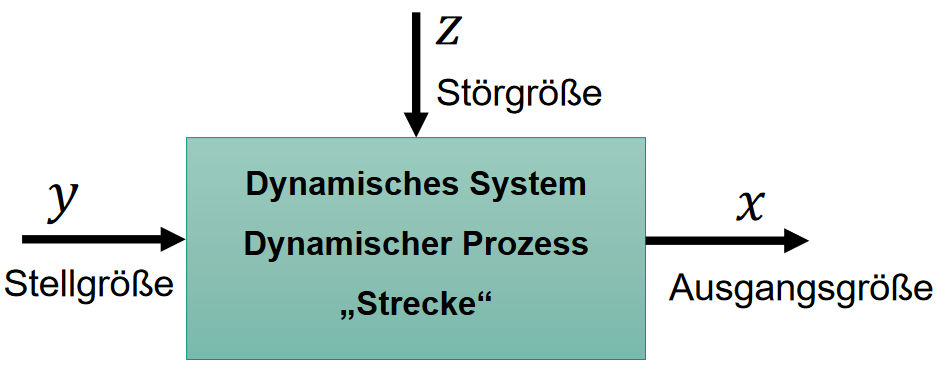
\includegraphics[width=0.4\textwidth]{images/regelung.png}
\end{center}

\textbf{Aufgabe}: Ausgangsgröße eines dynamischen Systems soll mittels der Stellgröße ein
Sollverhalten gegen den Einfluss einer Störgröße aufzeigen

\textbf{Prinzip}: Strecke ist laufend zu beobachten und Stellgröße ist derart zu verändern, dass trotz der Störgrößeneinwirkung die Ausgangsgröße an den gewünschten Verlauf angeglichen wird.

Eine Anordnung, die dies bewirkt heißt \textbf{Regelung}.\\

\textbf{Aufbau einer Regelung}:
\begin{center}
	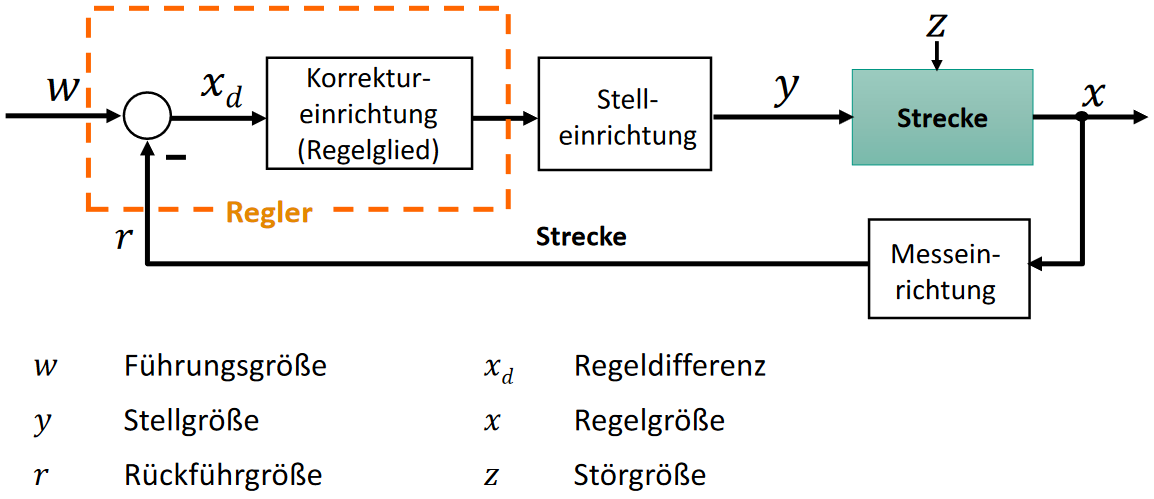
\includegraphics[width=0.7\textwidth]{images/regler-aufbau.png}
\end{center}
\bigskip
\textbf{Aufbau eines digitalen Signalverarbeitungssystems}:
\begin{center}
	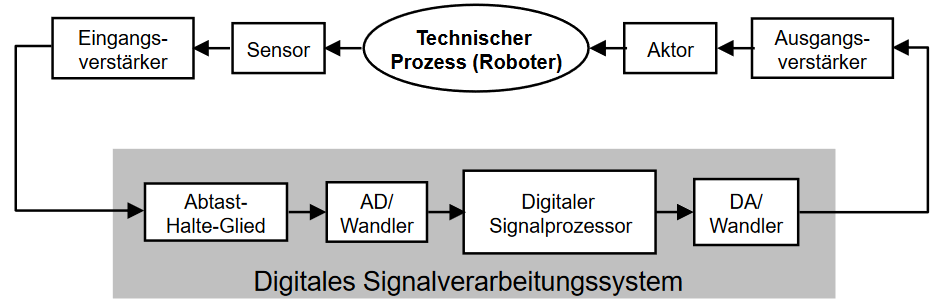
\includegraphics[width=0.7\textwidth]{images/signalverarbeitungssystem.png}
\end{center}
\begin{itemize}
	\item Abtast-Halte-Glied hält den abgetasteten Wert innerhalb einer Abtastperiode konstant
\end{itemize}
\bigskip
\textbf{Kontinuierliche und diskrete Signale}:
\begin{center}
	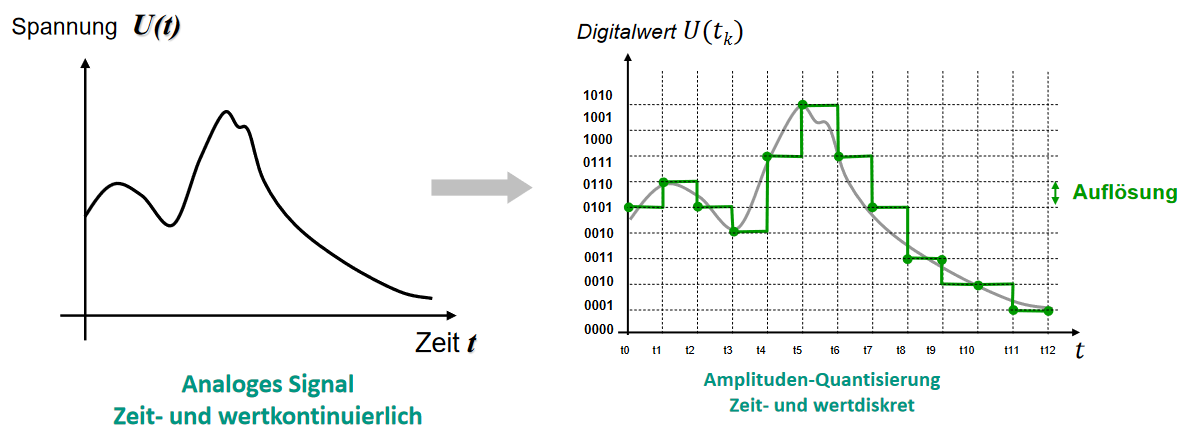
\includegraphics[width=0.9\textwidth]{images/ad.png}
\end{center}

\textbf{Beschreibung von Dynamischen Systemen}:
\begin{center}
	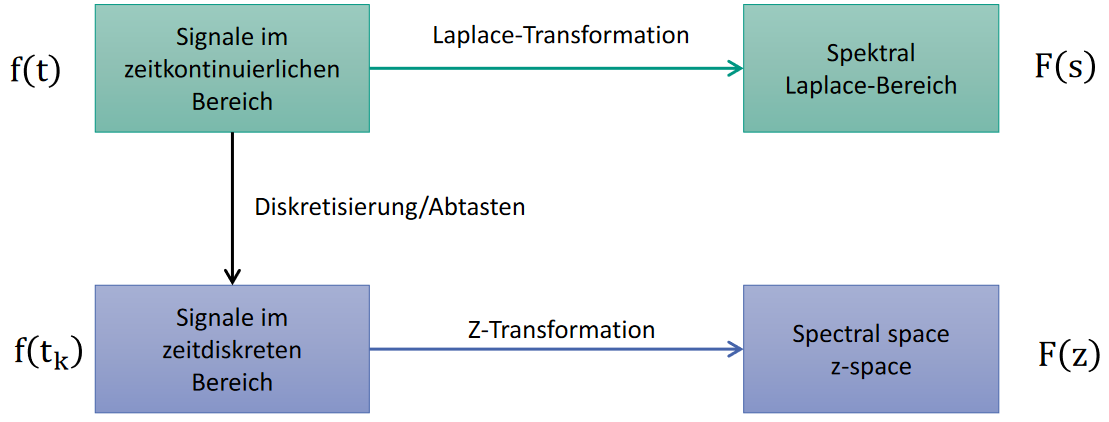
\includegraphics[width=0.7\textwidth]{images/trans.png}
\end{center}
\begin{itemize}
	\item Für Eingabesignal $u(t)$ und Ausgabesignal $y(t)$ werden die Laplace-Transformierten $U(s)$ und $Y(s)$ berechnet
	\item \textbf{Übertragungsfunktion} $G(s)=\frac{Y(s)}{U(s)}$
\end{itemize}
\bigskip
\textbf{Laplace-Transformation}:
\begin{itemize}
	\item $L\{f(t)\}=F(s)=\int\limits_0^{\infty} f(t)e^{-st}\, dt\qquad s\in\C; \quad f(t)=0,t<0$
	\item $L\{1\}=\frac{1}{s}, \quad L\{a\}=\frac{a}{s}, \quad L\{t\}=\frac{1}{s^2}$
	\item $L\{\dot{f}(t)\}=s\cdot F(s)-f(0)$
	\item $L\{\int\limits_0^{t}f(t)\,dt\}=\frac{1}{s}\,F(s)$
	\item $L\{e^{-\alpha t}\}=\frac{1}{s+\alpha}$
	\item Für Dirac-Impuls $\delta(t)$ ist $L\{\delta(t)\}=1$
	\item $L\{\alpha f_1(t)+\beta f_2(t)\}=\alpha F_1(s)+\beta F_2(s)$
\end{itemize}
Weiter Regeln siehe \textit{5/46-47}
\pagebreak

\textbf{Übertragungsglieder}:
\begin{center}
	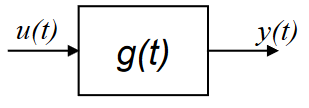
\includegraphics[width=0.2\textwidth]{images/uglied.png}
\end{center}
\begin{itemize}
	\item $Y(s)=G(s)\cdot U(s),\qquad G(s)\colon\text{Übertragungsfunktion}$ 
	\item $y(t)=g(t)*u(t)=\int\limits_0^{t} g(\tau)\cdot u(t-\tau)\, d\tau$, für $t>0$
	\item \textbf{Elementare Übertragungsglieder}: 
	\begin{center}
		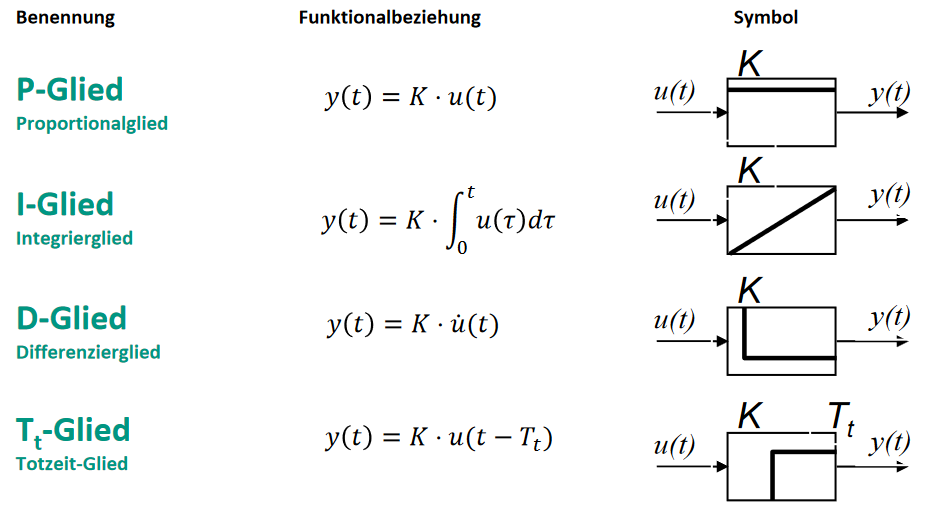
\includegraphics[width=0.7\textwidth]{images/pidt.png}
	\end{center}
 	\item \textbf{Umformregeln für Wirkungspläne}:
 	\begin{center}
 		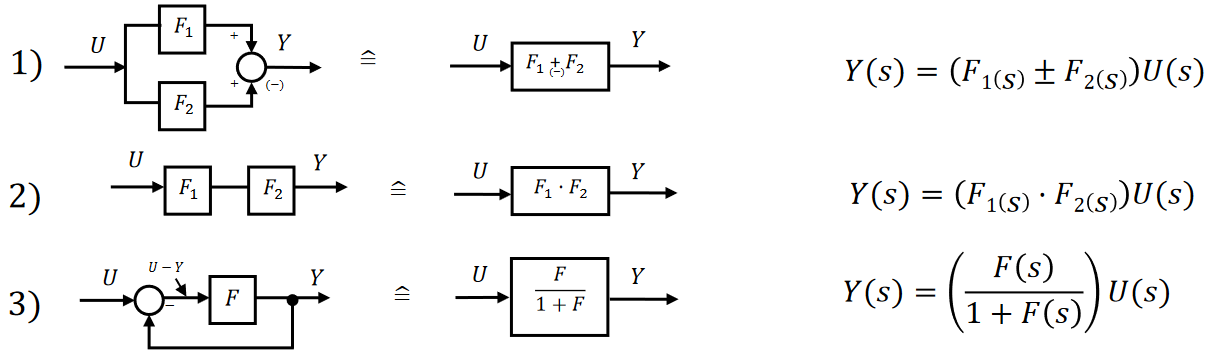
\includegraphics[width=0.8\textwidth]{images/uglied-rules.png}
 	\end{center}
\end{itemize}

\textit{Beispiel Erstellung des Strukturbildes des Regelkreis: 5/58-67}


